\section{问题二建模}
问题一提供了11:00:00至11:29:59在交叉路口驶入驶出车辆的时间、距离、位置等信息。在此基础上我们可以解决问题二。

\subsection{总流量和平均速度}

\subsubsection{定义与算法}
总流量:在采样时间段内驶离路口的车辆总数。

平均速度:各车辆行驶距离之和/各车辆行驶时间之和。

总流量只需,将所有驶离数据不为空的车辆计数加和即可,北口有194辆车通行,一辆未驶离;南口120辆均驶离;东口219辆,2辆未驶离;西口205辆,3辆未驶离。总流量为732辆。

平均速度的计算通过统计数据的进出时间长度求和/进出时间求和,即可得\textcolor{red}{总流量}。

\subsection{阻碍交通情况}

\subsubsection{道路概况}

下面引入一下交通问题中常用的变量及解释:


绿信比:绿信比是一个信号相位的有效绿灯时长与周期总时长之比。

信号周期:信号灯的各种灯色轮流显示一次所需要的时间。通常规定最短周期时间不得少于36秒。当交通需求较小时,信号周期则应较短,但一般不能小于P*15秒(P为相位数),以保证某一方向车辆及时安全通过路口。

进口道饱和流量:在一次连续的绿灯时间内,交叉口进车道上车队能够连续通过停车线的最多车辆数。

首先统计了信号灯的相位图,如下\ref{fig:p10}所示:
\begin{figure}[H]
    \centering
    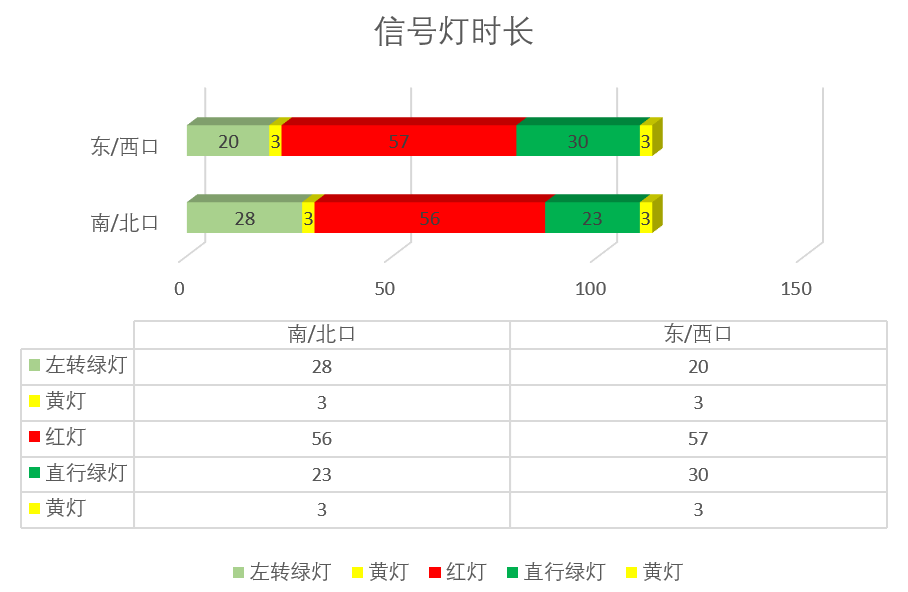
\includegraphics[scale=0.5]{figures/信号灯时长相位图.png}
    \caption{信号灯时长相位图}
    \label{fig:p10}
\end{figure}

东西方向与南北方向的信号周期均为113s,但显然信号灯的时长已经根据东西方向和南北方向车流量的不同进行了调整。南北方向左转车辆可能较多,东西方向直行车辆更多。这一特征可以在视频中显现。南北口的左转车辆略多于直行车辆,东西口则相反。同时也比较容易观察出的是北口车辆流量较大,其余路口车流稀少。

在我们查阅的论文中,对交叉路口交通信号优化控制,通常有以下2种角度:

(1)对信号周期进行优化;

(2)对相位信号(绿信比)进行优化;

我们若研究阻碍交通情况,也可以从这两个角度思考先考虑是不是信号周期整体时长不合理,无论是红灯还是绿灯都存在时长略长的情形;其次是考虑绿信比是否可以优化。此处我们作简要的说明,以北口11点钟的浙 98**8为例,在红灯倒计时56到38时,东西方向的停车等待的车辆大部分行驶完毕,剩下部分正好赶上绿灯而通行的车辆数量很少,那么直行的绿灯还有约10秒是被浪费了,对应的东西方向的绿灯时长过长,也代表着南北方向的红灯过长,故周期是不合理的,需要进行调整。相比之下,北口的车流量较大,直行和左转的时长基本恰好可以把等待的车辆放行结束。

通过观察可以发现,在路口通行的时候,无论是直行还是左转,大部分车辆都是在停车区或者待转区等待的车辆,恰好赶上绿灯的车辆为少数。也就是说,红灯的存在使得一部分车辆短暂停留在停车线,绿灯放行时,大部分车辆为等待的车辆,恰逢绿灯正常行驶的车辆是少数情况。\textcolor{red}{通过数据也可以观察出来,不需要停车的车辆比例相对于其他是很少的。(看数据再补全)}

\subsubsection{定义及结果}
本文对阻碍交通情况的定义为,在已经具备车辆正常通过路口的实时条件时,因为信号灯的存在而导致车辆不得不停车等待的情况为阻碍交通的情况。东西方向的车在绿灯时间内行驶结束,路口车辆被清空,南北方向的车辆理应正常行驶,但是需要等待红灯结束。同时也包含直行车辆清空,左转车辆仍需等待红灯才能左转的情形。


\begin{figure}[H]
    \centering
    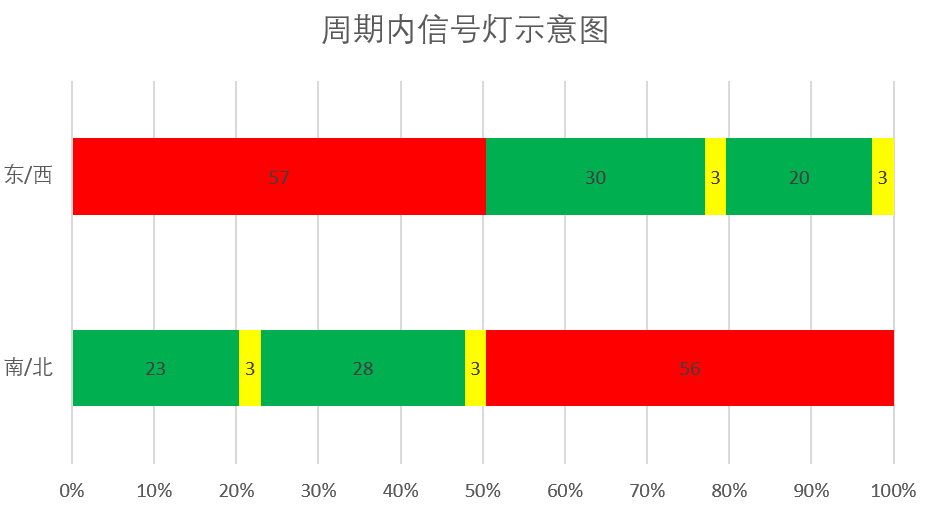
\includegraphics[scale=0.5]{figures/单周期信号灯示意图.png}
    \caption{单周期信号灯示意图}
    \label{fig:单周期}
\end{figure}

阻碍交通总时间的计算方法如下:
首先确定一个信号灯周期,分周期考虑每个周期内的阻碍交通时长,同时每个周期认为是相互独立此处以南北方向的直行绿灯亮起作为周期起点,具体示意如下\ref{fig:单周期},通过对周期进行划分,认为周期相互独立,再考虑各个周期内的阻碍时间的计算方法。

在最初级的处理中,我们只考虑临近时间区间的阻碍情况,例如东西方向的左转若有绿灯时间剩余,那么算作阻碍南北方向的直行;如果南北方向的直行绿灯有剩余,算作阻碍南北方向的左转;继而南北方向的左转会阻碍东西方向的直行。我们不考虑跨时间段阻碍,如果有车辆在南北方向红灯开始时就在左转停车区等待,那么东西方向的直行不仅会阻碍南北方向的直行,同时也会加长南北方向左转车辆的等待。但这种情况我们不考虑,只考虑直接相邻的时间区间的影响。

在计算阻碍时长的过程中,我们依次进行如下步骤:(1)记录南北方向直行车道,双向中最后一辆车辆驶离横线时的绿灯显示时间,记为$t1$,该时间算作阻碍南北方向左转车辆的时间;分别计算南北方向上自周期开始时至最后一辆车驶离时刻停留的车辆数,记为$x1$,$x_1\times t_1$则为南北方向直行阻碍南北方向左转的时间。
(2)记录南北方向左转双向车道中,最后一辆车驶离横线时绿灯显示时间,记为$t_2$, 该时间作为阻碍东西方向直行的车辆的阻碍时间;计算自周期开始时至最后一辆车左转驶离时刻时间内,停留的车辆数,记为$x_2$,用$x_2 \times t_2$作为南北方向左转阻碍东西方向直行的时间。
重复1、2步骤,但是是在计算东西方向的直行阻碍最左转,和东西方向左转阻碍南北方向直行。

对于车辆,在一个周期中,绿灯的主要放行目标定为,在红灯时刻到达等待绿灯的车辆。考虑“驶离横线时绿灯示数”这一指标,考虑同一周期内,同向行驶车辆,车辆行驶数量过半时,首次出现同向两车示数差异大于5秒以上,将前者剩余绿灯时间进行标记,调查其驶离路口时刻,该时刻认为不阻碍交通的绿灯开始时刻,考虑同时搜寻在另外方向上停车等待车辆。
车辆行驶玩